Художественное оформление Аны Кристины Чавес Калис.
\null
\vfill
\noindent{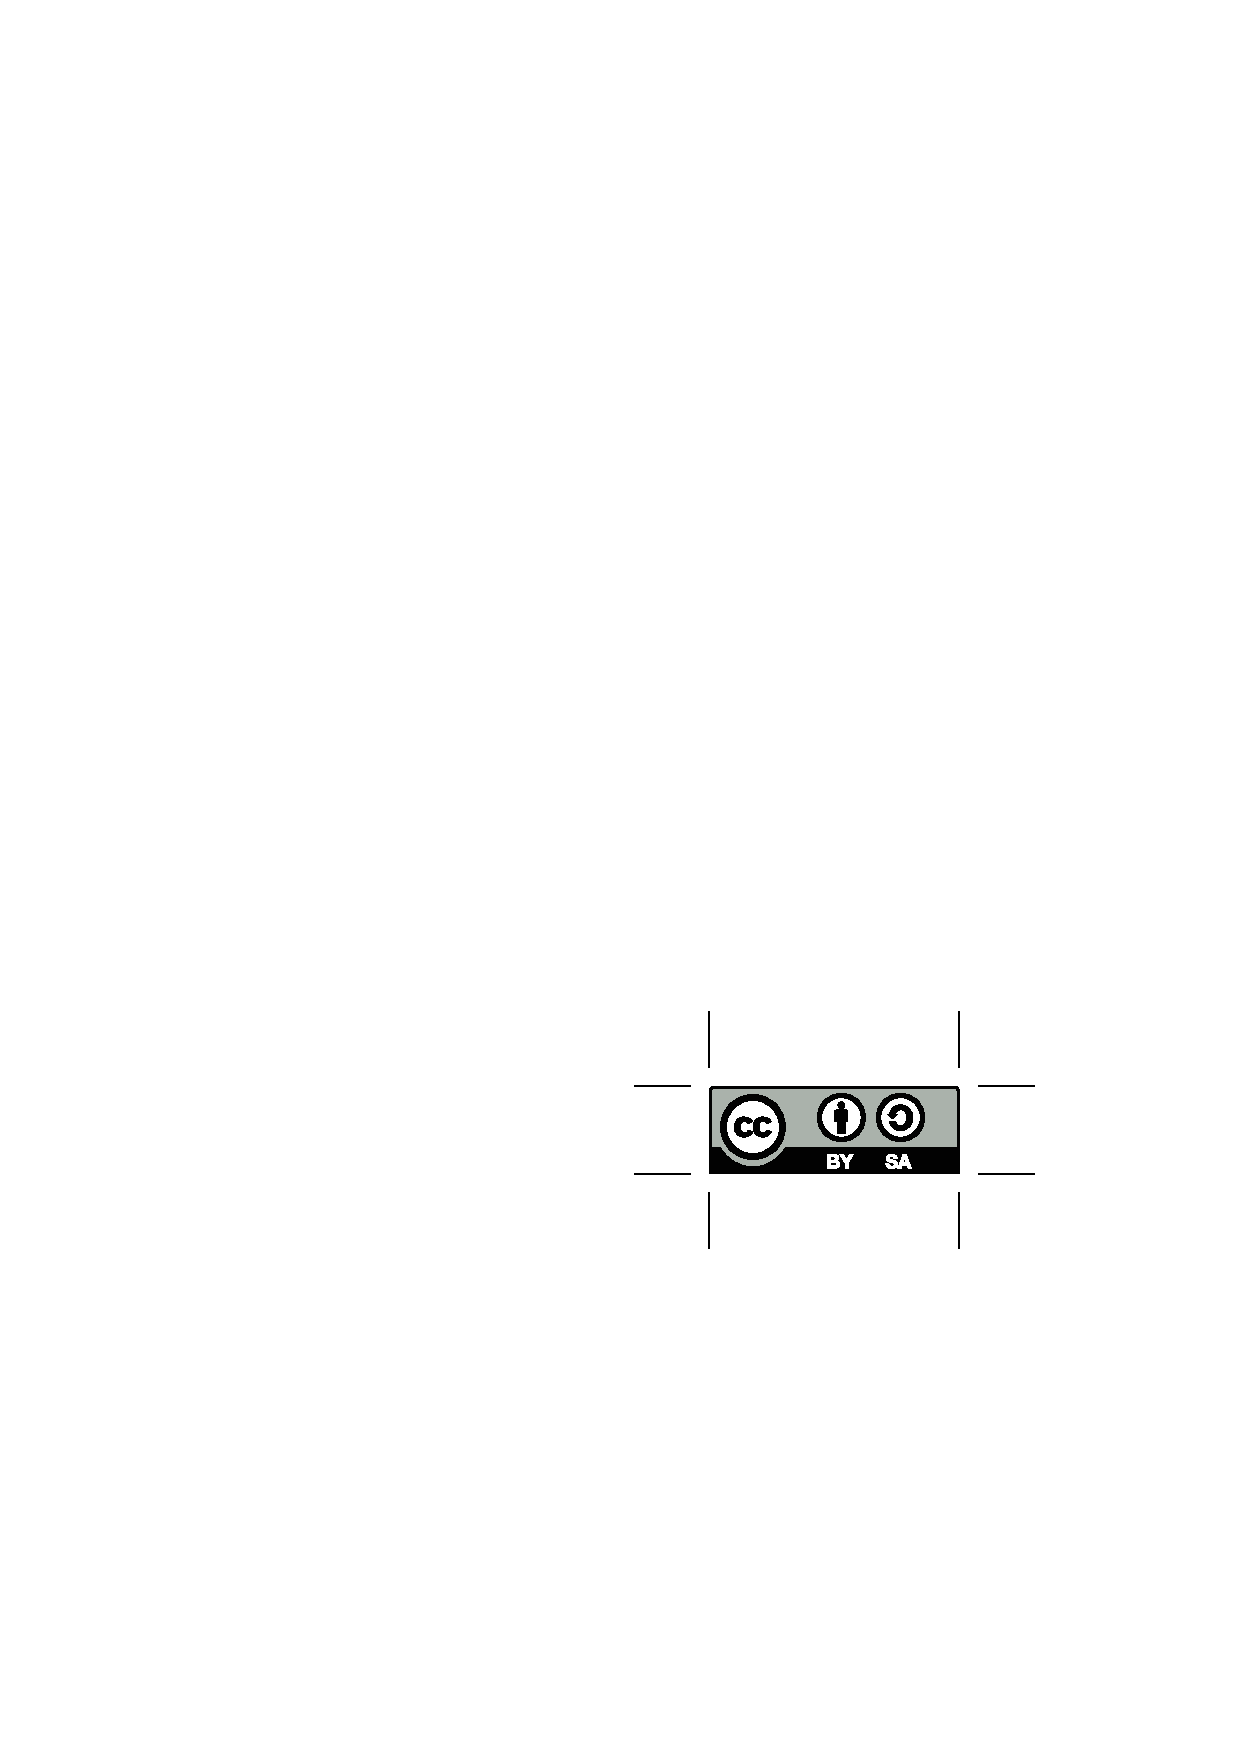
\includegraphics[scale=0.5]{pics/by-sa}
\vspace*{1mm}
\\
\hbox{\parbox{.8\textwidth}
{Это произведение распространяется на условиях лицензии CC BY-SA 4.0, с ней можно ознакомиться по ссылке
\texttt{https://creativecommons.org/licenses/by-sa/4.0}}}}


\thispagestyle{empty}
\newpage

%\phantomsection
\chapter*{Предисловие}
\addcontentsline{toc}{part}{Предисловие}
\thispagestyle{myheadings}
\markboth{ПРЕДИСЛОВИЕ}{ПРЕДИСЛОВИЕ}

Этот учебник рассчитан на тех, кто решил заниматься дифференциальной геометрией или же хочет найти вескую причину этого не делать.
Материала хватит на один семестр, и ещё останется.

Дифференциальная геометрия опирается на несколько разделов математики, включая
вещественный анализ,
теорию меры,
вариационное исчисление,
дифференциальные уравнения, топологию, элементарную и выпуклую геометрию.
В эту науку уйма входов, поэтому её и интересно, и трудно и преподавать, и изучать.

Гладкие кривые и поверхности дают важнейший источник примеров и идей дифференциальной геометрии.
Очень разумно хорошо разобраться в этой области прежде чем идти дальше --- не стоит спешить.

Мы делаем упор на задачи.
Доказательства элементарны, наглядны и почти строги;
мы пропускаем кое-что из других разделов, в основном тех, что обсуждаются в вводной части.
Мы сосредоточились на нескольких идеях, которые точно пригодятся в дальнейшем.
Поэтому обошли вниманием ряд тем, традиционно включаемых в вводные тексты;
например, мы почти не касаемся минимальных поверхностей и формул Петерсона --- Кодацци.

В то же время включены теоремы, которые обычно не обсуждаются в вводных курсах.

Первый пример --- теорема о луне в луже Владимира Ионина и Германа Пестова (\ref{thm:moon-orginal}).
Это наипростейший значимый пример так называемых теорем от локального к глобальному, которые лежат в основе всей дифференциальной геометрии;
он даёт хороший ответ на главный вопрос книги --- «Что такое дифференциальная геометрия?».
Другие примеры включают теорему о седловых графиках Сергея Бернштейна (\ref{thm:bernshtein}) и теорему о бесконечной двусторонней геодезической Стефана Кон-Фоссена (\ref{thm:cohn-vossen}).

Учебник основан на наших лекциях, прочитанных осенью 2018 года на MASS-программе Университета штата Пенсильвания.
Многие из тем использовались Юрием Бураго в его лекциях, читаемых в Ленинградском университете, когда первый автор был его студентом.
При написании мы подглядывали в учебники
Вильгельма Бляшке~\cite{blaschke},
Виктора Топоногова~\cite{toponogov-book},
и Алексея Чернавского \cite{chernavsky}, а также в лекции Сергея Иванова \cite{ivanov};
многие продвинутые упражнения взяты из \cite{petrunin2020}.
Последняя глава основана на вводном материале из книги Стефани Александер, Виталия Каповича и первого автора~\cite{alexander-kapovitch-petrunin2027}.
Мы хотим поблагодарить
Стефани Александер,
Юрия Бураго,
Берка Джейлана,
Нину Лебедеву,
Александра Лычака,
Бенджамина Маккея
и студентов нашего класса
за помощь.

Работа частично поддержана грантом NSF DMS-2005279 и грантом Фонда Саймонса  \#584781.

\begin{flushright}
Антон Петрунин и
\\
Серхио Замора Баррера.
\end{flushright}




